              
                %% bare_jrnl.tex
%% V1.4b
%% 2015/08/26
%% by Michael Shell
%% see http://www.michaelshell.org/
%% for current contact information.
%%
%% This is a skeleton file demonstrating the use of IEEEtran.cls
%% (requires IEEEtran.cls version 1.8b or later) with an IEEE
%% journal paper.
%%
%% Support sites:
%% http://www.michaelshell.org/tex/ieeetran/
%% http://www.ctan.org/pkg/ieeetran
%% and
%% http://www.ieee.org/

%%*************************************************************************
%% Legal Notice:
%% This code is offered as-is without any warranty either expressed or
%% implied; without even the implied warranty of MERCHANTABILITY or
%% FITNESS FOR A PARTICULAR PURPOSE! 
%% User assumes all risk.
%% In no event shall the IEEE or any contributor to this code be liable for
%% any damages or losses, including, but not limited to, incidental,
%% consequential, or any other damages, resulting from the use or misuse
%% of any information contained here.
%%
%% All comments are the opinions of their respective authors and are not
%% necessarily endorsed by the IEEE.
%%
%% This work is distributed under the LaTeX Project Public License (LPPL)
%% ( http://www.latex-project.org/ ) version 1.3, and may be freely used,
%% distributed and modified. A copy of the LPPL, version 1.3, is included
%% in the base LaTeX documentation of all distributions of LaTeX released
%% 2003/12/01 or later.
%% Retain all contribution notices and credits.
%% ** Modified files should be clearly indicated as such, including  **
%% ** renaming them and changing author support contact information. **
%%*************************************************************************


% *** Authors should verify (and, if needed, correct) their LaTeX system  ***
% *** with the testflow diagnostic prior to trusting their LaTeX platform ***
% *** with production work. The IEEE's font choices and paper sizes can   ***
% *** trigger bugs that do not appear when using other class files.       ***                          ***
% The testflow support page is at:
% http://www.michaelshell.org/tex/testflow/


% Please refer to your journal's instructions for other
% options that should be set.
\documentclass[journal,onecolumn,12pt]{IEEEtran}
%
% If IEEEtran.cls has not been installed into the LaTeX system files,
% manually specify the path to it like:
% \documentclass[journal]{../sty/IEEEtran}


\usepackage{amsmath}
\usepackage{caption}
\usepackage{mathtools}
\usepackage{subfigure}
\usepackage{url}
\usepackage{cite}
\usepackage[pdftex]{graphicx}
\usepackage{algorithmic}
\usepackage{array}
\usepackage{stfloats}

\hyphenation{op-tical net-works semi-conduc-tor}


\begin{document}
%
% paper title
% Titles are generally capitalized except for words such as a, an, and, as,
% at, but, by, for, in, nor, of, on, or, the, to and up, which are usually
% not capitalized unless they are the first or last word of the title.
% Linebreaks \\ can be used within to get better formatting as desired.
% Do not put math or special symbols in the title.
\title{CS391L Machine Learning\\ Assignment 1}


\author{Srinath~Tankasala,\\ st34546}





% The paper headers

\maketitle

% As a general rule, do not put math, special symbols or citations
% in the abstract or keywords.
\begin{abstract}

In this assignment, an overview of Independent Component Analysis (ICA) is presented and is applied to separate a mixture of sounds. A set of 5 different sources were taken and mixed to obtain a 5 different "microphone" recordings. The ICA algorithm was applied to retrieve the individual sounds and the retrieval quality was examined.
\end{abstract}

\section{Introduction}

%\begin{figure}[!t]
%\centering
%\includegraphics[width=2.5in]{myfigure}
% where an .eps filename suffix will be assumed under latex, 
% and a .pdf suffix will be assumed for pdflatex; or what has been declared
% via \DeclareGraphicsExtensions.
%\caption{Simulation results for the network.}
%\label{fig_sim}
%\end{figure}


%\begin{figure*}[!t]
%\centering
%\subfloat[Case I]{\includegraphics[width=2.5in]{box}%
%\label{fig_first_case}}
%\hfil
%\subfloat[Case II]{\includegraphics[width=2.5in]{box}%
%\label{fig_second_case}}
%\caption{Simulation results for the network.}
%\label{fig_sim}
%\end{figure*}

%\begin{table}[!t]
%% increase table row spacing, adjust to taste
%\renewcommand{\arraystretch}{1.3}
% if using array.sty, it might be a good idea to tweak the value of
% \extrarowheight as needed to properly center the text within the cells
%\caption{An Example of a Table}
%\label{table_example}
%\centering
%% Some packages, such as MDW tools, offer better commands for making tables
%% than the plain LaTeX2e tabular which is used here.
%\begin{tabular}{|c||c|}
%\hline
%One & Two\\
%\hline
%Three & Four\\
%\hline
%\end{tabular}
%\end{table}
The cocktail party problem is a classic application of ICA. There are many sound sources and focus needs to be given to the relevant ones and ignoring the others. In this problem we assume that we have recordings from different microphones of the same mixture of conversations. The cocktail party problem is solvable if the number of microphone recordings is equal to or greater than the number of sound sources in the room.

For the purposes of this assignment we mix the sounds so as to have equal number of "microphone" recordings. Additional microphone recordings may help increase the quality of the retrieved sounds, but that is not explored in this work.
\section{Mixing matrix}
We are given a test data set $U$ containing $n=5$ sound sources and $t$ number of samples. The aim is to mix these sounds to generate a pseudo microphone output $X$ of $m=5$ recordings. To do this we use a mixing matrix A. While there is no restriction on the choice of A, for consistency we choose one A for this whole report\\
\begin{flalign}
    X = AU, \text{A is mixing matrix of size (m,n)}
\end{flalign}
Hence $X$ is a m-by-t matrix of the mixed sound signals.
\section{Independent Component Analysis}

ICA decomposes a mixture of signals into its individual sources. This is different from Principal Component Analysis which tries to find the dominant vector components in the given dataset. Our goal is to find the "un-mixing" matrix 'W' of size n-by-m.\\
\begin{flalign*}
    X = AU\\
    \text{determine W s.t.,}\\
    WA = I,\\
    \therefore U = WX
\end{flalign*}
We use an algorithm to find an estimate of the matrix $W$ called the maximum likelihood estimate, that is denoted by $\hat{W}$. This method is explained in the next section.\\
\subsection{Maximum Likelihood Estimation of Unmixing matrix:}
There are several methods available in literature that can be used to calculate the unmixing matrix $W$, \cite{} for example uses a SVD (singular value decomposition) methods to calculate the matrix W. There are advantages and disadvantages to the available approaches. For example, the SVD approach involves calculation of the Eigenvalues of $XX^T$ which may be slow if the number of microphone inputs (m) is large.
The Maximum Likelihood Estimate (MLE) of $W$ is calculated by maximizing the parameters of W to match the mixed data X. To do this, the following definition is used for the likelihood of the mixture X:

\begin{equation}
    p(x=X) = p_x(X) = p_u(U)\cdot|W| = \prod_{i=1}p_i(u_i)|W|    
\end{equation}

where, $p_u(U)$ is the probability density function of the independent source signals, and $p_i(u_i)$ is the probability density of the $i_{th}$ source component\\

Since we have $t$ samples of all mixtures in X, we can calculate $P_x(X)$ as:


\begin{equation}
    L(W) = \prod_{j=1}^t\prod_{i=1}^np_i(w_i^Tx_j)|W|
    \label{eq:likelihood def}
\end{equation}
where, $x_j$ is the $j^{th}$ column of X.\\
Thus our goal is to maximize $L(W)$ over all $W$, i.e.:
\begin{equation}
    \max_{W\epsilon R^{(n,m)}} L(W)
    \label{eq:optimality-eqn}
\end{equation}
Given that the probability density function is always positive, we can maximize $L(W)$ by maximizing the log likelihood function. The reason for maximizing log likelihood is because, taking log of $L(W)$ changes the product terms in $W$ into summation terms, i.e.:

\begin{eqnarray}
    \ln{(L(W))} =& \sum_{j=1}^t\sum_{i=1}^n\ln{(p_i(w_i^Tx_j)|W|)}&\\
     =& \sum_{j=1}^t\sum_{i=1}^n\ln{(p_i(w_i^Tx_j)}& + \sum_{i=1}^n\ln(|W|)\\
     \therefore \ln{(L(W))} =& \sum_{j=1}^t\sum_{i=1}^n\ln{(p_i(w_i^Tx_j)}& + t\ln{(|W|)}
     \label{eq:simplified loglike}
\end{eqnarray}
We can simplify equation \ref{eq:simplified loglike} further as:
\begin{equation}
    \frac{1}{t}\ln{(L(W))} = E\left[\sum_{i=1}^n\ln{(p_i(w_i^Tx_j))}\right] + \ln{(|W|)}
    \label{eq:log-like-Exp}
\end{equation}
where E[] is the expectation/mean observation. \\
Here we introduce the concept of the cumulative density function (cdf). The cumulative density function $g(X)$ is the integral of the pdf, and gives the net probability of the function having a value below X. Thus the pdf $p(X)$ is simply the derivative of $g(X)$. Thus equation \ref{eq:log-like-Exp} becomes,\\
\begin{equation}
    \frac{1}{t}\ln{(L(W))} = E\left[\ln{(g'(WX)}\right] + \ln{(|W|)}
    \label{eq:log-like-Exp-cdf} 
\end{equation}

There are many algorithms that are available for maximizing the the log-likelihood function. Gradient descent algorithm is a popular approach to maximize $L(W)$. Since we maximize with respect to W, the gradient is taken accordingly, i.e.:
\begin{equation}
    \frac{1}{t}\frac{\partial}{\partial W}\ln(L(W)) = E\left[\frac{\partial}{\partial W}(\ln{(g'(WX)})X^T\right] + \frac{\partial}{\partial W}\ln{(|W|)} = E\left[\frac{\partial}{\partial W}(\ln{(g'(WX)})X^T\right] + \left[W^T\right]^{-1}
\end{equation}
\subsection{Gradient Descent:}
The gradient descent algorithm is a iterative algorithm which can be used to minimize or maximize a function. If the function being optimized is convex in nature then the gradient descent converges to the function extremum. Proving the convexity of the function $L(W)$ is beyond the scope of this report and it has not been shown here. Gradient descent starts at an initial guess point $\hat{W}_1$ and updates it by moving along the function gradient evaluated at that point. Thus a gradient descent applied to find $W$ results in:

\begin{equation}
    \hat{W}_{k+1} = \hat{W}_k + \eta\cdot\left(\frac{1}{t}\frac{\partial}{\partial W}\ln(L(W))\right)_{W=\hat{W}_k} = \hat{W}_k + \eta\cdot\Delta W
\end{equation}
where, $\hat{W}_k$ is the estimate of the $W$ matrix after the $k^{th}$ iteration of the gradient descent algorithm. The starting point, i.e. $\hat{W}_1$ is assumed random, however for the sake of consistency of results shown in this report, the value of $\hat{W}_1$ is taken fixed. $\eta$ is the "learning rate" of the gradient descent algorithm and should be adjusted to achieve convergence.\\
Now the gradient term contains an inverse operation  for the $W^T$ matrix which is computationally expensive to calculate. Thus the gradient step can be conditioned by multiplying it with $W^TW$. This does not affect it's convergence to the optimum. It would involve a lot of algebra to show that the optimality of equation \ref{eq:optimality-eqn} is unaffected by making the above change. For brevity of this report, this has been omitted and it is encouraged to refer the class notes. Hence,
\begin{eqnarray}
    \Delta W = E\left[\frac{\partial}{\partial W}(\ln{(g'(WX)})X^T\right] W^TW + \left[W^T\right]^{-1} W^TW \\
    \therefore    \Delta W = \left(E\left[\left(\frac{\partial}{\partial W}(\ln{(g'(WX)})\right)(WX)^T\right] W + W\right)_{W=\hat{W}_k}
    \label{eq:delta W simplified}
\end{eqnarray}

To facilitate the gradient descent algorithm, it will be ideal to choose a $cdf$ that is differentiable for all possible values of $WX$ and is also easy to calculate. With that in mind, the $cdf$ is defined as
\begin{equation*}
    g(WX) = \frac{1}{1+e^{-WX}}
\end{equation*}
this function is differentiable for all $WX$ and is bounded between 0 and 1. It is easy to show that the corresponding $pdf$, i.e. the derivative of $g$ is given by:
\begin{equation*}
    g'(WX) = g(WX)(1-g(WX))
\end{equation*}
With this simplification, we can plug the above derivative into equation \ref{eq:delta W simplified} to get,
\begin{equation}
    \Delta W = \left(\left(E\left[(1-2g(WX))(WX)^T\right] + I \right)W\right)_{W=\hat{W}_k}
\end{equation}
The final algorithm can be summarized as:
\begin{enumerate}
    \item Start with an intial guess of the W matrix, i.e. $\hat{W}_1$  
    \item Calculate matrix $Z_k$ which is given by $g(\hat{W}_kX)$
    \item Calculate $\Delta W$ using $W_k$ as $\left(E\left[(1-2Z_k)(\hat{W}_kX)^T\right] + I \right)\hat{W}_k$
    \item Update the estimate as $\hat{W}_{k+1} =\hat{W}_k + \eta\cdot\Delta W$
    \item Check for convergence by seeing if $||\Delta W||/||W||$ is below the tolerance value, if not then return to step 2
\end{enumerate}

\section{Results and Discussion}
The original source signals were extracted from the 'sounds.mat' file. They were used to obtain the $U$ matrix. The mixing matrix can be any random 5x5 matrix that is full rank (5). For consistency between multiple runs, the signals were mixed with the following mixing matrix:\vspace{12pt}\\
$A = [[0.5, 1, 0.2, 1, 0.3];[0.5, 0.5, 0.2, 0.6, 0.1];[0.8, 0.4, 0.5, 0.5, 0.31];[0.5, 0.4, 0.5, 1, 1];[0.2, 0.7, 0.7, 0.1, 0.3]]$\vspace{12pt}\\
The mixed signals matrix (X) was obtained by multiplying A and U. \\
For the gradient descent algorithm, the learning rate was set to $\eta = 0.01$ and the tolerance limit for the relative norm, i.e. $||\Delta W||/||W||$, was set to $10^{-6}$. The algorithm finished in 6979 iterations and was able to successfully isolate the individual components/sources.
\begin{figure}[h]
\centering
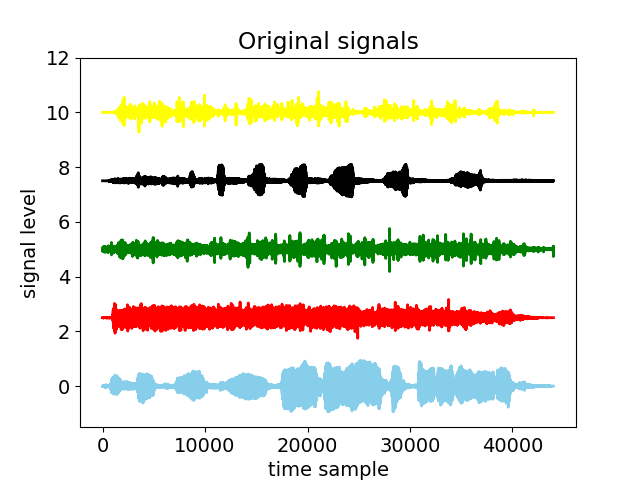
\includegraphics[width=4in]{images/Original_signals.png}
\caption{Original signals in ascending order (y-offset is for plotting purposes)}
\label{fig:orig_sigs}
\end{figure}

\begin{figure}[h]
\centering
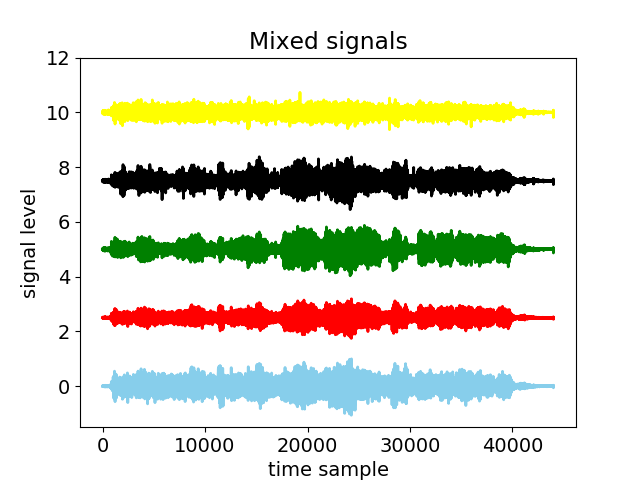
\includegraphics[width=4in]{images/Mixed_signals.png}
\caption{Mixed signals in ascending order (y-offset is for plotting purposes)}
\label{fig:mix_sigs}
\end{figure}

If $W$ is a solution to equation \ref{eq:optimality-eqn}, then so is $a\cdot W$ where $a$ is any scalar. This means that the solution is not unique and depends on our chosen starting point $\hat{W}_1$. Hence, for consistency between multiple runs, $\hat{W}_1$ was chosen as a fixed value.\\
Once we obtain the best estimate $\hat{W}$, we can retrieve the estimate of the original signals by multiplying with X, i.e. $\hat{U} = \hat{W}X$, where $\hat{U}$ is the retrieved estimate\\
\begin{figure}[h]
\centering
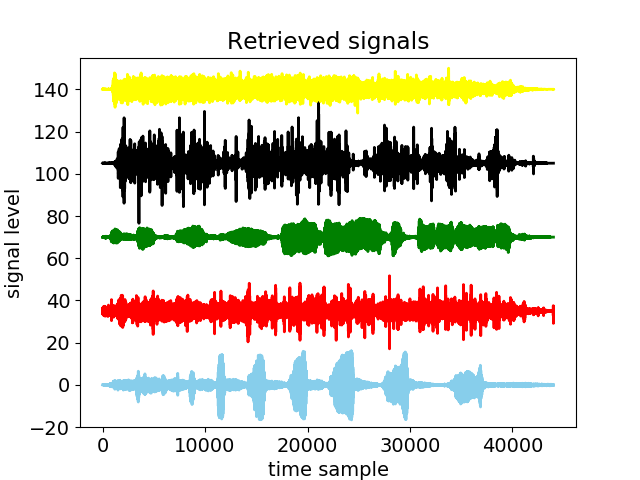
\includegraphics[width=3.8in]{images/Retrieved_signals.png}
\caption{Retrieved signals in ascending order (y-offset is for plotting purposes), notice the magnitudes}
\label{fig:ret_sigs}
\end{figure}

It can be seen from Fig \ref{fig:ret_sigs}, that the retrieved signals are scaled and not in the same order as the source signals. Since we actually know what is the mixing matrix $A$, we can obtain the scaling factor and order of signals from the product $\hat{W}\cdot A$. This would not be possible normally as A would be unavailable. In such cases, the sources have to manually matched. Then all signals in the retrieved estimate would have their peaks normalized between [-1,1].
%\subsection{Performance of ICA}
The performance of the ICA algorithm can be measure by how well the retrieved signals correlate with the original sources, as shown below, 
\begin{figure}[h]
\centering
\includegraphics[width=3.8in]{{"images/Correlation_signals"}.png}
\caption{Correlation between source signals and their corresponding recovered signals}
\label{fig:correl_imgs}
\end{figure}\\
As can be seen in Fig \ref{fig:correl_imgs}, the algorithm improves its estimate as the number of iterations increase. Also notice that the correlation asymptotically reaches -1 or 1. This means that the rate of convergence slows down as iterations increases. The quality of the retrieval can also be visualized by overlaying the source signal and the scaled retrieved signal.

\begin{figure}[h]
\centering
\includegraphics[width=4in]{{"images/Homer_Simpson_audio"}.png}
\caption{Comparison of source and retrieved Homer Simpson audio}
\label{fig:homer}
\end{figure}\\


\section{Conclusion}
In conclusion, 


\end{document}